\documentclass[12pt, letterpaper]{article}
\usepackage{amsmath}
\usepackage{amssymb}
\usepackage{hyperref}
\usepackage{graphicx}

\DeclareMathOperator*{\argmin}{argmin}

\title{Decision analysis of toy NAO}
\author{Daniel P. Rice}
\date{February 2023}

\begin{document}

\maketitle

\begin{abstract}
    This document outlines the decision analysis of the recurring decision problem with two simple hypotheses: threat vs. non-threat, and two actions: flag, and wait for more data.
    See \href{https://docs.google.com/document/d/1CsTdi18Nt4UGAkmTSUeFLiZsvC4N4-b_AdL7-Gddu_M/edit?usp=sharing}{the Feb 2023 all-hands memo} for background.
\end{abstract}

\tableofcontents

\section{Model}

We consider a toy model of threat monitoring with a stream of data.
In this model, we collect a data series ${X_1, X_2, \ldots}$ in order to determine whether a sequence is a threat (hypothesis $T$) or a non-threat (hypothesis $NT$).
Each time we collect data, we can choose to flag the sequence for costly follow-up or to wait for the next datapoint.

Our goal is to determine the optimal decision rule for flagging versus waiting, given the data that we have observed so far.
We consider two costs: the cost ($c$) of flagging a non-threat, and the cost ($d$) of delaying for more data if there is threat.
We treat the data collection itself as a fixed cost.

With these costs, we have a loss function at time $i$:
\begin{equation}
    L_i =
    \begin{tabular}{l c c}
        & not-threat & threat \\
        flag & $c$ & $0$ \\
        wait & $L_{i+1}$ & $d + L_{i+1}$.
    \end{tabular}
    \label{eq:loss}
\end{equation}
Note the recursive nature of the loss: if we choose to wait for more data, our loss at time $i$ includes the future loss $L_{i+1}$.

Our objective is to minimize the expected loss before we've collected any data:
\begin{equation}
    \mathbb{E}[L_0] = (1-p_0)\mathbb{E}[L_0 | NT] + p_0\mathbb{E}[L_0 | T],
    \label{eq:loss_cond}
\end{equation}
where $p_0 = \mathbb{P}[T]$ is our prior probability of a threat.

Whenever we collect data $X_i$, we update our prior according to Bayes rule.
Let $P_i$ be our posterior probability having seen data $\{X_1,\ldots,X_i\}$.
If the $X_i$ are IID (conditional on $T$ or $NT$), with likelihood functions $p(X|T)$ and $p(X|NT)$, we have Bayesian updates:
\begin{equation}
    P_{i+1} = \frac{P_{i} p(X_{i+1}|T)}{P_{i} p(X_{i+1}|T) + (1 - P_{i}) p(X_{i+1}|NT)}.
\end{equation}
The posterior probability contains all of the information we have at time $i$,
so we can specify a decision rule: flag if $P_i \ge p_{t}$, wait otherwise.
Here $p_t$ is the threshold posterior probability for flagging.
We will choose the threshold to minimize the expected loss.

It is convenient to work with log-odds rather than probabilities.
Letting $Q_i = \log P_i \ (1 - P_i)$, we have a transformed update rule:
\begin{equation}
    Q_{i+1} = Q_i + \log \frac{p(X_i | T)}{p(X_i | NT)}.
\end{equation}
Thus, the log-odds $Q$ are a random walk with a jump size distribution determined by the log likelihood ratio of the data.

In many circumstances, the distribution of the log likelihood ratio is approximately Gaussian.
For concreteness, we'll consider a case where it is exactly Gaussian.
Let the data be normally distributed so that:
\begin{align}
    X_i \sim \mathcal{N}(I[T], \tau^{-1})
\end{align}
where $I(T)$ is an indicator function and in the inverse variance, $\tau$ measures the precision of the data.
(Note that as long as the variance is the same under the two hypotheses, we can write any normally distributed data in this form.)
In this case,
\begin{align}
    Q_{i+1} - Q_{i} \sim N(\pm \tau / 2, \tau),
\end{align}
with a positive mean if $T$ and negative mean if $NT$.
That is, $Q$ updates on average in the correct direction and the updates are larger and have a smaller coefficient of variation when the data is more precise (larger $\tau$).

We now have all the pieces we need to calculate the conditional expected losses in Eq.~\ref{eq:loss_cond}.
If our current log-odds is $q$, then before we collect data $X_i$, we can calculate the expected loss by marginalizing over possible updates:
\begin{align}
    \mathbb{E}[L_{i-1}(q) | NT] & = \int_{-\infty}^{q_t} K_{NT}(q, q') \mathbb{E}[L_{i}(q')| NT]  dq' + c \int_{q_t}^{\infty} K_{NT}(q, q') dq' \\
    \mathbb{E}[L_{i-1}(q) | T] & = \int_{-\infty}^{q_t} K_{T}(q, q') \mathbb{E}[L_{i}(q')| T]  dq' + d.
\end{align}
The integration kernel $K(q, q')$ is the probability density of updating $Q$ from $q$ to $q'$.
Because our model is time-homogeneous, we can set the expectations on both sides equal to one another.
This gives us 
\begin{align}
    \mathbb{E}[L(q) | NT] & = c u_{NT}(q_t - q) \\
    \mathbb{E}[L(q) | T] & = d u_{T}(q_t - q) 
\end{align}
where the functions $u$ solve the Fredholm integral equations:
\begin{align}
    u_{NT}(x) & = \int_{0}^{\infty} K_{NT}(t - x) u_{NT}(t) dt + \int_{-\infty}^{0} K(t - x) dt 
    \label{eq:fredholm_nt} \\
    u_{T}(x) & = \int_{0}^{\infty} K_{T}(t - x) u_{T}(t) dt + 1.
    \label{eq:fredholm_t}
\end{align}
(In our model, $K(q, q')$ is translation-invariant, so we can write it as $K(q' - q)$.)
Note that these are both special cases of the linear Fredholm equation of the second kind:
\begin{align}
    u(x) &= \int_0^{\infty} K(t - x) u(t) dt + f(x)
\end{align}

Putting everything together an minimizing the loss, gives us the condition for the optimal threshold:
\begin{equation}
    (1 - p_0) c u_{NT}'(q_t - q_0) + p_0 d u_{T}'(q_t - q_0) = 0,
    \label{eq:optimum}
\end{equation}
where $q_0 = \log \frac{p_0}{1-p_0}$ is the prior log-odds.

\section{Asymptotics}

Eqs.~\ref{eq:fredholm_nt} and \ref{eq:fredholm_t} are difficult to solve in general.
In this section, we consider asymptotic solutions in two limits.
First we look at the limit where the data is very good at distinguishing between threats and non-threats, so that we expect to cross the theshold posterior in just a few updates if there is a threat.
Then, we look at the opposite limit, where it may require many updates to cross the threshold, either because the data is noisy or because our prior probability is very low.

\subsection{Case 1: Few updates}

When our data is strong (i.e. $\tau \gg 1$ in our Gaussian example), updates tend to move us reliably in the correct direction.
In this case, we can use the Liouville-Neumann series solution to the integral equation.
For
\begin{align}
    u(x) &= \int_0^{\infty} K(t - x) u(t) dt + f(x) \\
    u(x) &= f(x) + \sum_{n=1}^{\infty} \int_0^{\infty} K_n(t - x) f(t) dt
    \label{eq:ln_series}
\end{align}
where $K_1 = K$ and $K_n = \int K(t - x) K_{n-1}(t) dt$.
One can think of the $n$-th term in the series as representing the contribution to the loss from the $(n+1)$-th update.
If the data is strong, the terms rapidly shrink because with high probability we've either crossed the threshold in the threat case or moved very far from it in the non-threat case.
Thus, we can get good accuracy by considering a truncated series.
Fig.~\ref{fig:large_updates} shows the expected cost of delay if there is a threat strong data.

\begin{figure}
    \centering
    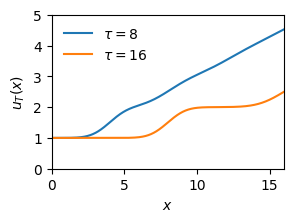
\includegraphics{u_T}
    \label{fig:large_updates}
    \caption{The expected cost of delay if there is a threat with large $\tau$. Note the contribution of discrete updates at intervals of the average update size, $\tau / 2$, which smooth out for larger $x$.}
\end{figure}

Substituting Eq.~\ref{eq:ln_series} into Eq.~\ref{eq:optimum}, and use the Gaussian model, we get a condition for the optimal threshold:
\begin{align}
    (1 - p_0) c \sum_{n=1}^{\infty} \frac{1}{\sqrt{n\tau}} \phi\left(\frac{q_t - q_0 + n \tau / 2)}{\sqrt{n\tau}} \right) & = 
    p_0 d \sum_{n=1}^{\infty} \frac{1}{\sqrt{n\tau}} \phi\left(\frac{q_t - q_0 - n \tau / 2)}{\sqrt{n\tau}} \right)
\end{align}
where $\phi$ is the standard Gaussian density.
This equation is somewhat inscrutable, but if $q_t - q_0 < \tau / 2$, we can truncate the series at the first term (considering only one update) and solve for $q_t$.
This gives us a posterior odds threshold
\begin{align}
    \frac{p_t}{1-p_t} & \approx \frac{c}{d}.
\end{align}
Using the optimal decision rule, we have
\begin{align}
    \mathbb{E}[L(q_t)] \approx p_0 d.
\end{align}
This tells us that in the strong data limit where we only expect to have to collect data about one time:
\begin{enumerate}
    \item The decision threshold is determined by the ratio of the cost of false positives to the cost of a single delay.
    \item The loss is dominated by the cost of that single delay times the prior probability that there is a threat.
\end{enumerate}
Note that this is the same result we got in the all-hands memo in the stong-data limit of the case where we only had the option to collect data once, which makes sense.

\subsection{Case 2: Many updates}

We now turn to the case where we have to consider more than a few updates, either because our data is weak and does not reliably update us in the correct direction or because our prior is very far from the threshold.
In this case, the Liouville-Neumann series (Eq.~\ref{eq:ln_series}) converges slowly, so we need a different approximation.
Since we're concerned with behavior far from the threshold, we'll look for the asymptotic behavior of $u(x)$ as $x \to \infty$.

First, we look at expected cost in the non-threat case. 
Here, $f(x) \to 0$ rapidly, so the dominant balance for large $x$ is given by
\begin{align}
    u(x) \sim \int_0^{\infty} K(t - x) u(t) dt.
\end{align}
This is a homogeneous equation, so we can try the ansatz $u(x) \sim A e^{\lambda}$.
Substituting and taking the limit $x \to \infty$, we get:
\begin{align}
    \int_{-\infty}^{\infty} K(s) e^{\lambda s} ds \to 1.
\end{align}
This is an eigenvalue problem in $\lambda$, which can be solved by recognizing that the left-hand side is the moment-generating function for the update size distribution $K$.
In our Gaussian model, we have
\begin{align}
    \frac{\tau}{2} \lambda + \frac{\tau}{2} \lambda^2 = 0.
\end{align}
The trivial solution $\lambda = 0$, can be discarded because it implies a constant cost of false positives as $x\to \infty$, which does not make any sense.
This leaves us with $\lambda = -1$, and thus
\begin{align}
    u_{NT}(x) \sim A_{NT}(\tau) e^{-x}.
\end{align}

We have only to determine the behavior of the constant $u_{NT}(0) = A_{NT}$, which depends on $\tau$.
For small $\tau$, $A_{NT} \to 1$ (because the updates converge to an unbiased Brownian motion, which returns to zero with probability 1).
For large $\tau$, we can use the Liouville-Neumann series as above to get $A_{NT}(\tau) \sim \Phi(-\frac{\sqrt{\tau}}{2})$, where $\Phi$ is the standard normal CDF.

\begin{figure}
    \centering
    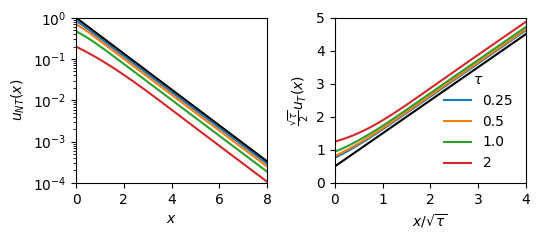
\includegraphics{small_updates}
    \label{fig:small_updates}
    \caption{The expected losses with small updates. Black lines show the asymptotic behavior for large $x$ and small $\tau$.}
\end{figure}

The same approach gives the expected cost in the threat case:
\begin{align}
    u_{T}(x) \sim \frac{2}{\tau} x + A_{NT}(\tau).
\end{align}
For small $\tau$, $A_{T}(\tau) \sim \frac{const.}{\sqrt{\tau}}$.
(The the diffusion timescale is $\frac{1}{\sqrt{\tau}}$, so we can think of this as a coarse-graining of $\frac{1}{\sqrt{\tau}}$ updates.)

For large $\tau$, $A_{T} \to \frac{1}{2}$, which is consistent with the large $\tau$ analysis above.

[Aside: We can get more terms of the asymptotic series above by iteration. To get the next term, substitute the current series into the right-hand side Fredholm equation.]

Given these values for the conditional expected losses, we can find the threshold log-odds:
\begin{equation}\frac{p_t}{1 - p_t} \to \frac{\tau c}{2 d}\end{equation}
and expected loss:
\begin{equation}E[L] \to p_0 d \frac{q_t - q_0}{\tau / 2}\end{equation}
Here $q_t - q_0$ is the distance between your prior log-odds and your threshold and each update moves $q$ in the right direction by $\tau / 2$ on average.
So the expected loss is the per-update delay cost $d$ times the number of updates we expect to need.

The strong-data limit is consistent with these results, but takes into account the discreteness of the updates in that case.

\section{Numerics}

In this section, we outline a numerical approach to calculating the conditional expected loss, which should hold in general.
Recall that for both $T$ and $NT$, our expected loss is determined by the solution to a Fredholm equation of the second kind:
\begin{equation}
    u(x) = \int_{0}^{\infty} K(x, t) u(t) dt + f(x).
\end{equation}
We can approximate the integral using Gauss-Laguerre quadrature:
\begin{equation}
    u(x) \approx \sum_{j=1}^{n} w_j \exp(t_j) K(x, t_j) u(t_j) + f(x) \label{eq:quad}.
\end{equation}
The nodes $t_j$ and weights $w_j$ are given by a standard formula, and the $\exp$ term is required to cancel the implicit weight function $\exp(-x)$.

Evaluating both sides of the equation at the quadrature nodes gives linear system for $u_i = u(x_i)$:
\begin{equation}
    u_i \approx \sum_{j=1}^{n} w_j \exp(x_j) K(x_i, x_j) u_j + f_i.
\end{equation}
We solve the system for $u_i$.

Finally, we can get a continuous approximation for $u(x)$ by substituting $u(t_j) = u_j$ in the right-hand side of Eq.~\ref{eq:quad}.

\end{document}
